%!TEX root = research_proposal.tex

\pagenumbering{arabic}
\setcounter{page}{1}

\chapter{Introduction}

Maintenance activities are known to be costly and challenging \cite{Pressman2005}. Studies have shown that the cost of software maintenance can reach up to 70\% of the overall cost of the software development process \cite{HealthSocial2002}.
By ``maintenance activity'' we mean any change to software beyond its first release or iteration; i.e. development of software where there is already an existing system that is to be changed.
This is the broadest possible meaning of the term.
It includes adding new features, creating new iterations, as well as classic adaptive and corrective maintenance.

The difficulties encountered by maintainers are various.
In large software project, difficulties are partially attributable to the fact that the software are created, distributed and maintained globally.
Developers and users are scattered across the globe.

Consequently, maintainers can hardly have complete knowledge over the software at hand.
Yet, such knowledge will be an asset to avoid known mistakes, programming errors and improve the software.

In the last decade, source code revision control system and project tracking systems have grown to contain hundreds of thousands of revision, bug and crash report per project.
Naturally, this plethora of data pushed researchers across the world to conduct hundreds of studies in several active research fields: bug reproduction, bug triaging, duplicated bug identification, bug comprehension, bug re-production.

In order to support software maintenance, researchers and developers started to mine software repository.
Software repository contains the each modification made to the software and related issues.

Mining software repository---the science of interpreting software artifacts---is perhaps one of the most active research field today.
The reason is that their analysis provides useful insight that can help with many maintenance activities such as bug fixing \cite{Weiss2007,Saha2014}, bug reproduction \cite{Artzi2008,Jin2012,Chen2013}, fault analysis \cite{Jiang2012,Jin2013}, bug prediction \cite{Hovemeyer2007}, etc.

A great length of efforts have been conceded by the mining software repository community to create tools and approaches ranging from simple text-pattern matching to complex predictive models.
These tools are often automatically tested and verified in laboratory\cite{Lewis2013}.
Indeed, manually testing and validating industrial-sized repository for each iteration of a given algorithm is counterproductive.
This automation of experiment allows researchers to improve their approaches and compare tools to each others.
The current state-of-the-art approach can always be improved by new and more complex technics\cite{Hovemeyer2004}.
\\
Yet, one question remains:  Is it useful to {\bf human} maintainers?
\\
This simple question has been studied by researchers and companies alike (noticeable examples \cite{Lewis2013,Foss2015,Layman2007,Ayewah2007,Ayewah2008,Johnson2013,Norman2013, Lopez2011}).
Of course, the results of such studies are not binary and can be difficult to interpret.
Nevertheless, it has been discovered that although human maintainers agree that such tools are beneficial, false positives and the way in which the warnings are presented, among other things, are barriers to use\cite{Johnson2013}.
In addition, human maintainers agree with some of the characteristics that maintenance-oriented tools should have \cite{Hovemeyer2004, Lopez2011, Lewis2013}:

\begin{itemize}
	\item Actionable messages. Presenting a warning about bug-proneness of a given line is not enough.
	Clear actions to improve the source code should be provided
	\item Obvious reasoning. The conditions that led to a given warning should be understandable by the maintainer.
	If the conditions are hidden in complex statistical models, then maintainers cannot review them and will find it difficult to trust the tool.
	\item Scaling. Industrial sized project contains thousand files and dependencies which can be updated many times a day.
	Maintenance-oriented tools should not hinder the productivity of maintainers.
	\item Contextualization. Warnings and messages should always be  with respect to the project at hand and not generic rules.
	\item Integration. Developers and maintainers are overwhelmed by the amount of existing tools.
	Yet, their daily use three different kinds of tools.
	An integrated development environment, a versioning system and a project tracking system to produce, version and manage their software, respectively.
	Maintenance-oriented tools should fit in the existing ecosystem rather than complexifying the deployment process.
\end{itemize}

To tackle these limitations, we introduce the notion of pragmatic software maintenance where maintenance activities are dealt with in a sensible and realistically way that is based on practical rather than theoretical considerations.

In the following sections, we describe the thesis contribution and the proposal outline.

\section{Problems in the Literature\label{sec:pb-litterature}}

\begin{itemize}

		\item {\bf Problem 1}: The literature contains numerous papers about tools that improve the overall software quality with static \cite{Dangel2000, burn2003checkstyle, Hovemeyer2007, Moha2010} and dynamic \cite{Nayrolles,Nayrolles2013a,Palma2013} analysis.
		At a few exceptions (such as \cite{Lopez2011, Montandon2013}), these tools do not account for the context of the project.
		By context, we refer to past versions, reports, comments or any direct and indirect software artifact that could help provide precise steps to resolve a given warning.

		\item {\bf Problem 2}: Tools aiming to ease maintenance processes do not integrate themselves seamlessly in the  five steps of maintenance: acknowledge a report or a task, create a branch, fix or enhance source code, test, mark branch as ready	\cite{Kamiya2002a, Nayrolles, Nayrolles2013a, Jeffrey2009, Chen2013, Gavrilov2013, Jin2012, Nessa2008, Dallmeier, Nayrolles2015a, demange2013, Jiang2007, Iss2009}.
		Indeed, most of the tools are plain-old tools, at the exception of the IDE plugins \cite{Kamiya2002a, Hovemeyer2007}, that maintainers have to install and update manually.
		Then, for each completed task, the tools have to be started and their results analyzed: false positive discarded and warning messages decrypted.
		This among other things, are barriers to their broad adoption \cite{Johnson2013,Lewis2013}.

		\item {\bf Problem 3}: As shown by Figure \ref{fig:scholar}, the proportion of empirical studies and studies based on mining software repositories regarding to software quality have increased exponentially since 2005 (\cite{Kim2011a,Lee2011a,Sun2011,Bhattacharya2011,Tian2012a,Zimmermann2012, Shang2013, Chen2014, McIntosh, Hemmati2015} are some noticeable examples).
		Yet, the field lack of a clear taxonomy to be able to compare approaches efficiently and replicate experiments\cite{Hassan2008,Godfrey2009}.

	\begin{figure}[h!]
	  \centering
	  	    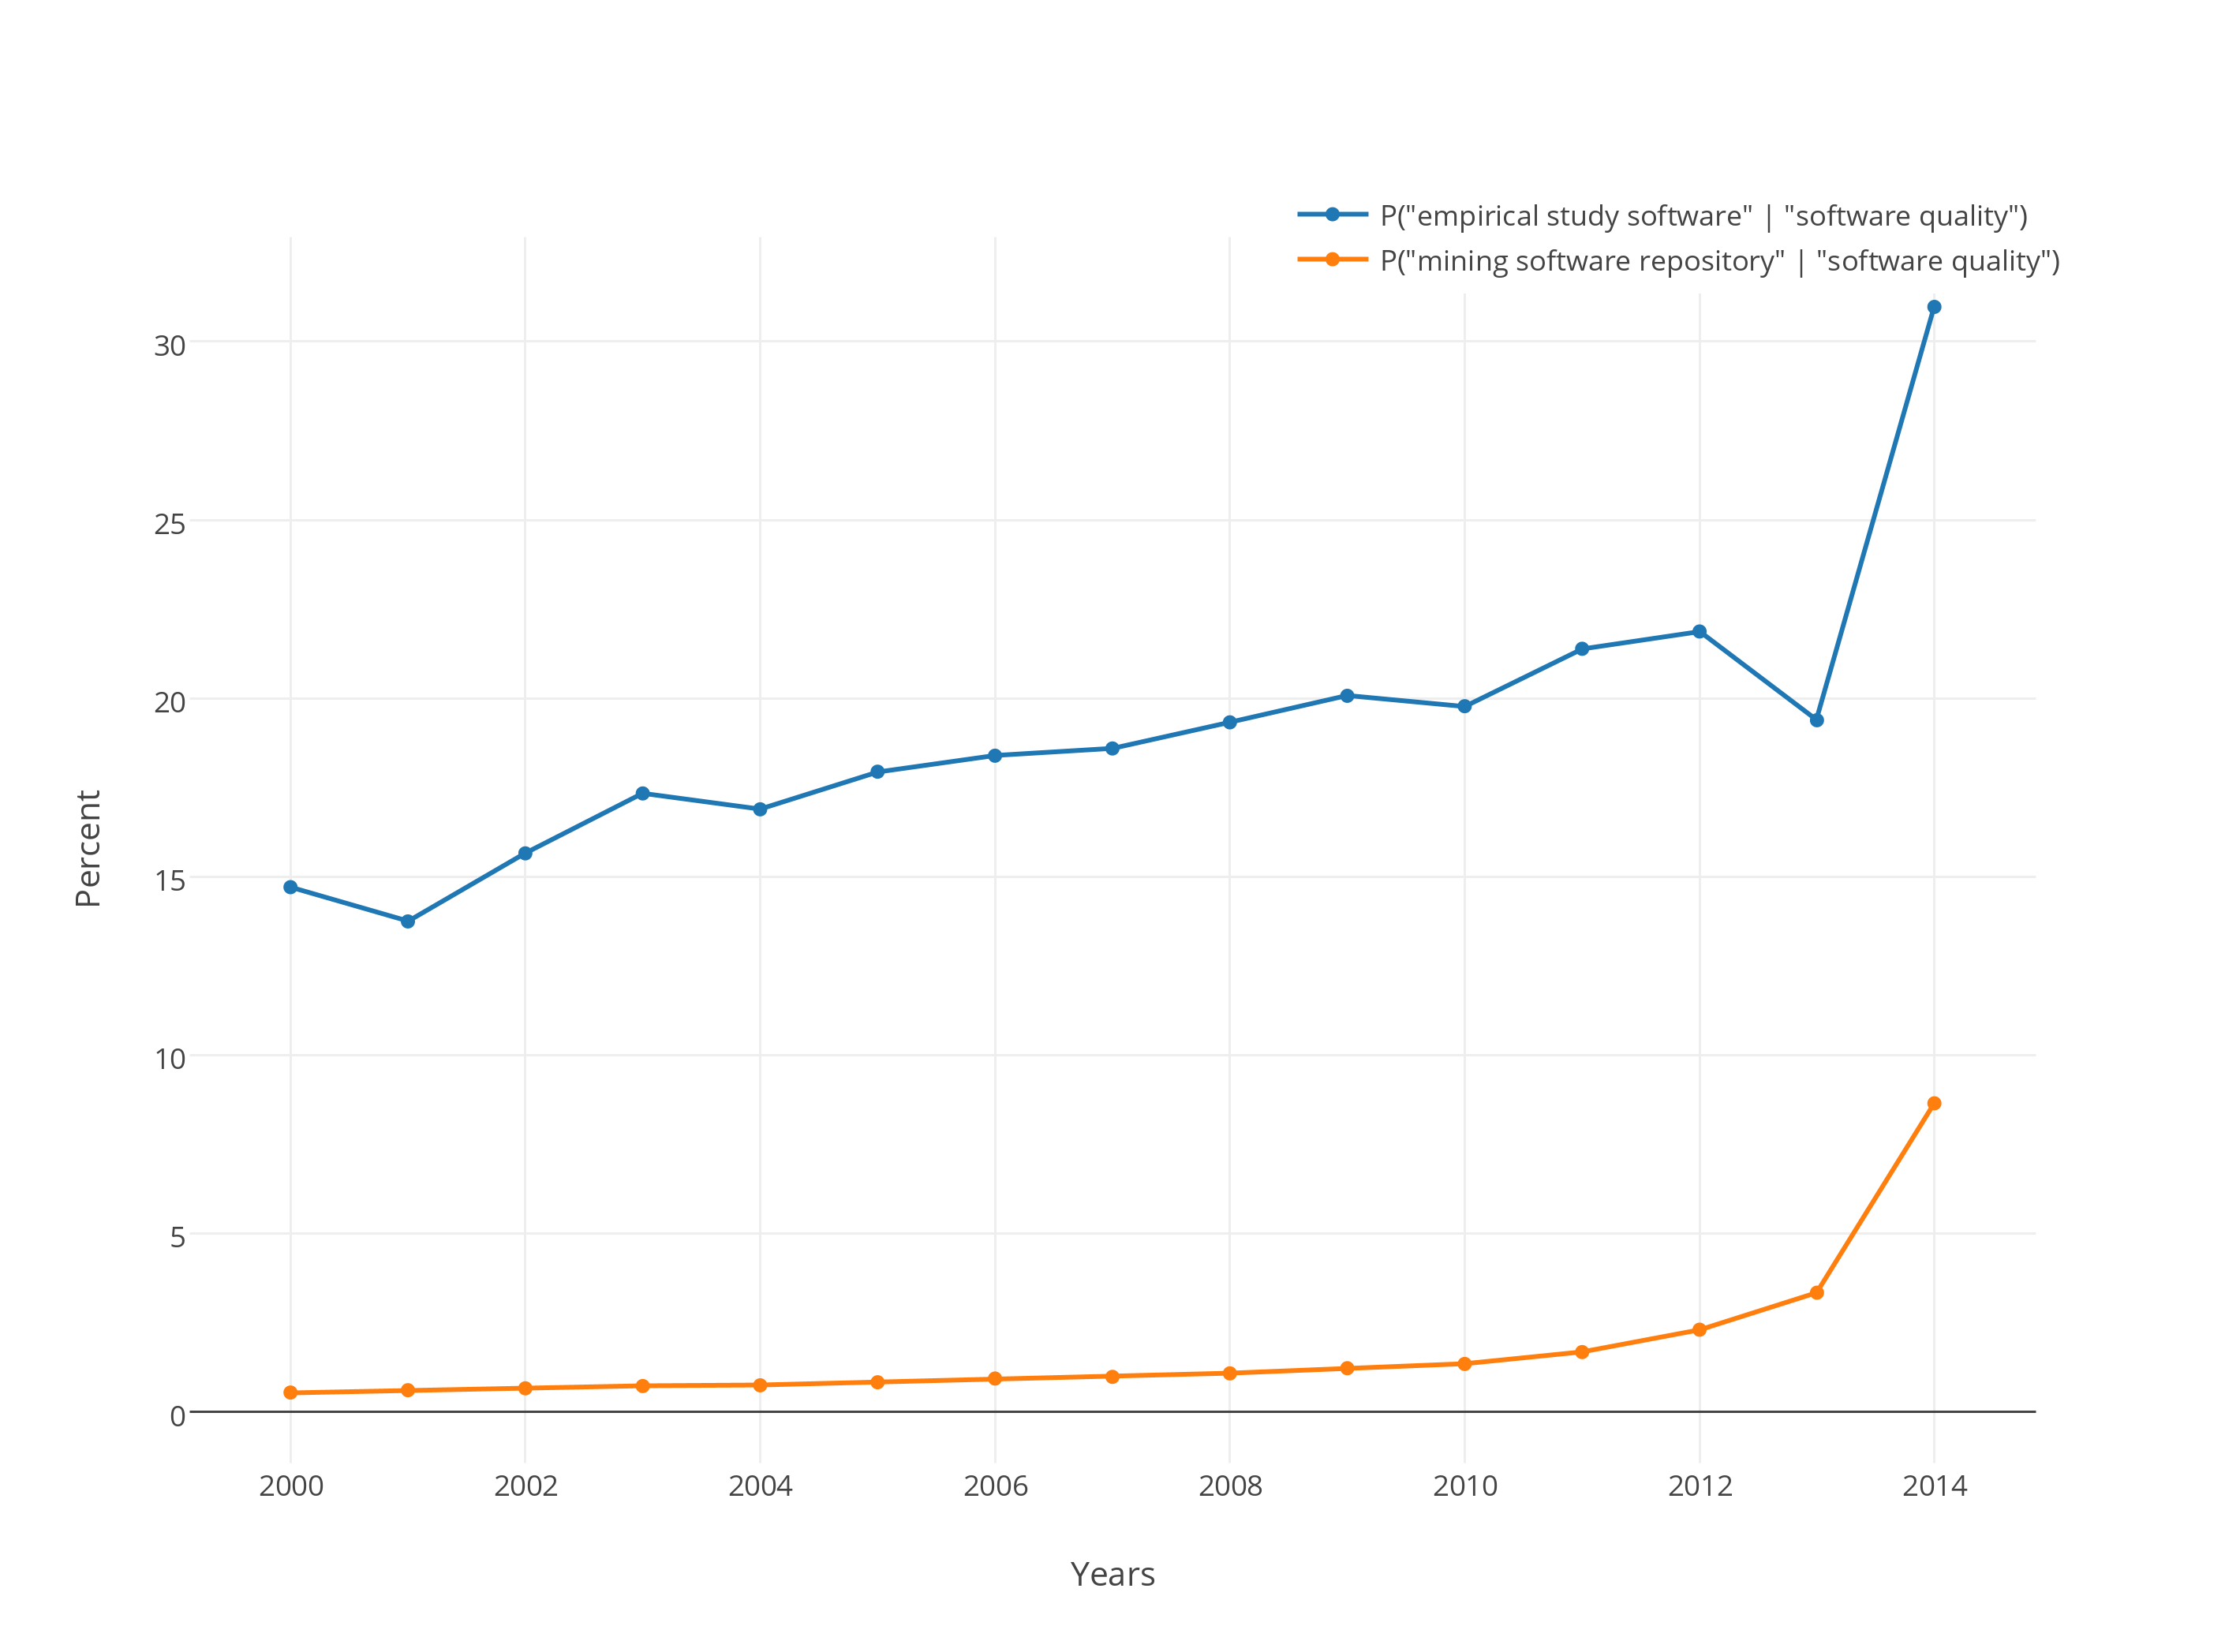
\includegraphics[scale=0.7]{media/scholar.png}
	    \caption{Proportion of papers containing ``Empirical Study'' or ``Mining software repository'' with regards to the paper in Software quality indexed by Google Scholar	\label{fig:scholar}}
	\end{figure}

\end{itemize}

\section{Research Contributions\label{sec:objective-thesis}}

In this section, we present our different research contributions.
The main research contributions we aim to achieve are:

\begin{itemize}
	\item An analysis of existing techniques aiming to support software maintenance.
	\item The notion of pragmatic software maintenance and a dedicated framework.
	\item A taxonomy to classify the research on software maintenance.
\end{itemize}

The remainder of this section elaborates on these contributions.
The next section presents the proposal outline.

\subsection{An analysis of Existing Techniques Aiming to Support Software Maintenance}

We have observed that many tools and technics aiming to support software maintenance try to improve on the current state-of-the-art technic in terms of precision or recall.
However, these authors of these technics rarely consider to the usability of their work in industrial environments.

Understanding the barriers to adoption of these technics will help us create technics that maintainers are more likely to use.

\subsection{Pragamatic Software Maintenance}

We introduce the notion of pragmatic software maintenance where maintenance activities are dealt with in a sensible and realistically way that is based on practical rather than theoretical considerations.

We introduce {\tt PASMAST} (PrAgmatic Software Maintenance At verSioning Time) a framework for pragmatic software maintenance.
{\tt PASMAST} is composed of five tools interfacing themselves seamlessly with maintainers' processes.
More specifically, {\tt PASMAST} can:
\begin{itemize}
	\item Create steps to reproduce crashes.
	\item Prevent clone insertion.
	\item Provide recommendation on code modification.
	\item Prevent error insertion.
\end{itemize}

\subsection{A Taxonomy to Classify the Research on Software Maintenance}

We want to provide a way to classify the research related to defaults in software maintenance.
Such taxonomy will allow researchers to specialize in classes of defects and to be able to compare accurately their approaches with other, very much like the taxonomy that exists for clones detection\cite{CoryKapser}.

From the bug handling perspective, if we can develop a
way to detect such related bug reports during triaging then we can achieve considerable time savings in the way bug reports are processed, for example, by assigning them to the same developers.
We also conjecture that detecting such related bugs can help with other tasks such as bug reproduction.
We can reuse the reproduction of an already fixed bug to reproduce an incoming and related bugs.

The objective of our taxonomy is not to propose a way to
detect such related bug reports or how we can take advantage
of them to improve the bug handling process, but it is to
introduce a new way of grouping bugs into types that we
believe can facilitate the bug handling process.

\section{Outline\label{sec:outline}}

The remaining chapters of this proposal are:

\begin{itemize}
	\item Chapter \ref{chap:relwork} - {\it Background \& Related work}.
	In this chapter, we present major works on the fields related to our research. Namely, crash reproduction, reports and source code relationships, crash prediction and clone detection.
	\item Chapter \ref{chap:pasmast} - {\it PASMAST: An Open Source Framework for Pragmatic Software Maintenance} presents our framework for pragmatic software maintenance.
	\item Chapter \ref{chap:aggreating} - {\it Aggregating Version Control and Project Management Systems} presents our attempt to aggregate versioning and project managements systems.
	More specifically, we present two approaches: one providing an API to retrieve software artifacts belonging to versioning and project management systems and one to reproduce field crash.
	\item Chapter \ref{chap:clone-detection-pragmatic} {\it Using clone detection for pragmatic software maintenance}.
	This chapter describes three approaches---and their preliminary results---to ease software maintenance activities by using clone detection technics.
	\item Chapter \ref{chap:taxonomy} {\it A taxonomy to classify the research}. Classifying the research on fields related to software maintenance is essential for reproduction and improvement purposes.
	In this chapter, we present a taxonomy classifying the relationship between report and source-code modifications.
	\item Chapter \ref{chap:plan} {\it Remaining Work to Complete the
Thesis} presents  the remaining work and a publication plan.
\end{itemize}
